
\section{讨论}
\label{sec:discussion}

上述机制将注意力从提示本身转移到提示所引发的推理状态区域。当学生的推演过程到达教师能够提供有效监督的区域时，输入才具有价值。陈述问题只是达到这些区域的一种方式。这一视角引出了两个更广泛的问题：输入本身需要包含多少任务内容？为什么相同的one-shot情景在OPD和RLVR下表现不同？我们通过分析内容稀疏和跨领域输入来探讨这些问题，随后与one-shot RLVR进行受控对比。

\subsection{输入作为状态生成器}
\label{sec:template}

状态生成器视角认为，如果输入仍能引发教师可监督的轨迹，则任务内容可能是不必要的。我们通过一个以 \texttt{<think>} 结尾的空用户回合、相同模板搭配简单领域系统提示，以及来自 WildChat~\citep{zhao2024wildchat} 的通用领域查询（图~\ref{fig:template-examples}）来验证这一预测。WildChat 数据集包含 \(192{,}824\) 个主要为英文的通用对话、创意写作、角色扮演和改写类查询。保守性启发式仅将 \(0.17\%\)  标记为与数学相关，\(2.63\%\)  标记为与代码相关。

\begin{figure}[t]
\centering
\begin{minipage}[t]{0.485\textwidth}
\begin{tplbox}{(a) Base template}
\begin{tplinput}
\ttfamily\scriptsize\raggedright \tplctrl{<|begin\_of\_sentence|>}\tplrole{<|用户|>}\tplthink{思考}\tplesc{\textbackslash n}
\end{tplinput}
\end{tplbox}
\end{minipage}\hfill
\begin{minipage}[t]{0.485\textwidth}
\begin{tplbox}{(b) System template --- Code}
\begin{tplinput}
\ttfamily\scriptsize\raggedright \tplctrl{<|begin\_of\_sentence|>}解决编程竞赛问题。从标准输入读取，向标准输出写入。\tplrole{<|User|>}\tplthink{<|think|>}\tplesc{\textbackslash n}
\end{tplinput}
\end{tplbox}
\end{minipage}
\\[4pt]
\caption{用于OPD训练输入的两个内容稀疏模板。}
\label{fig:template-examples}
\end{figure}

\begin{figure}[t]
\centering
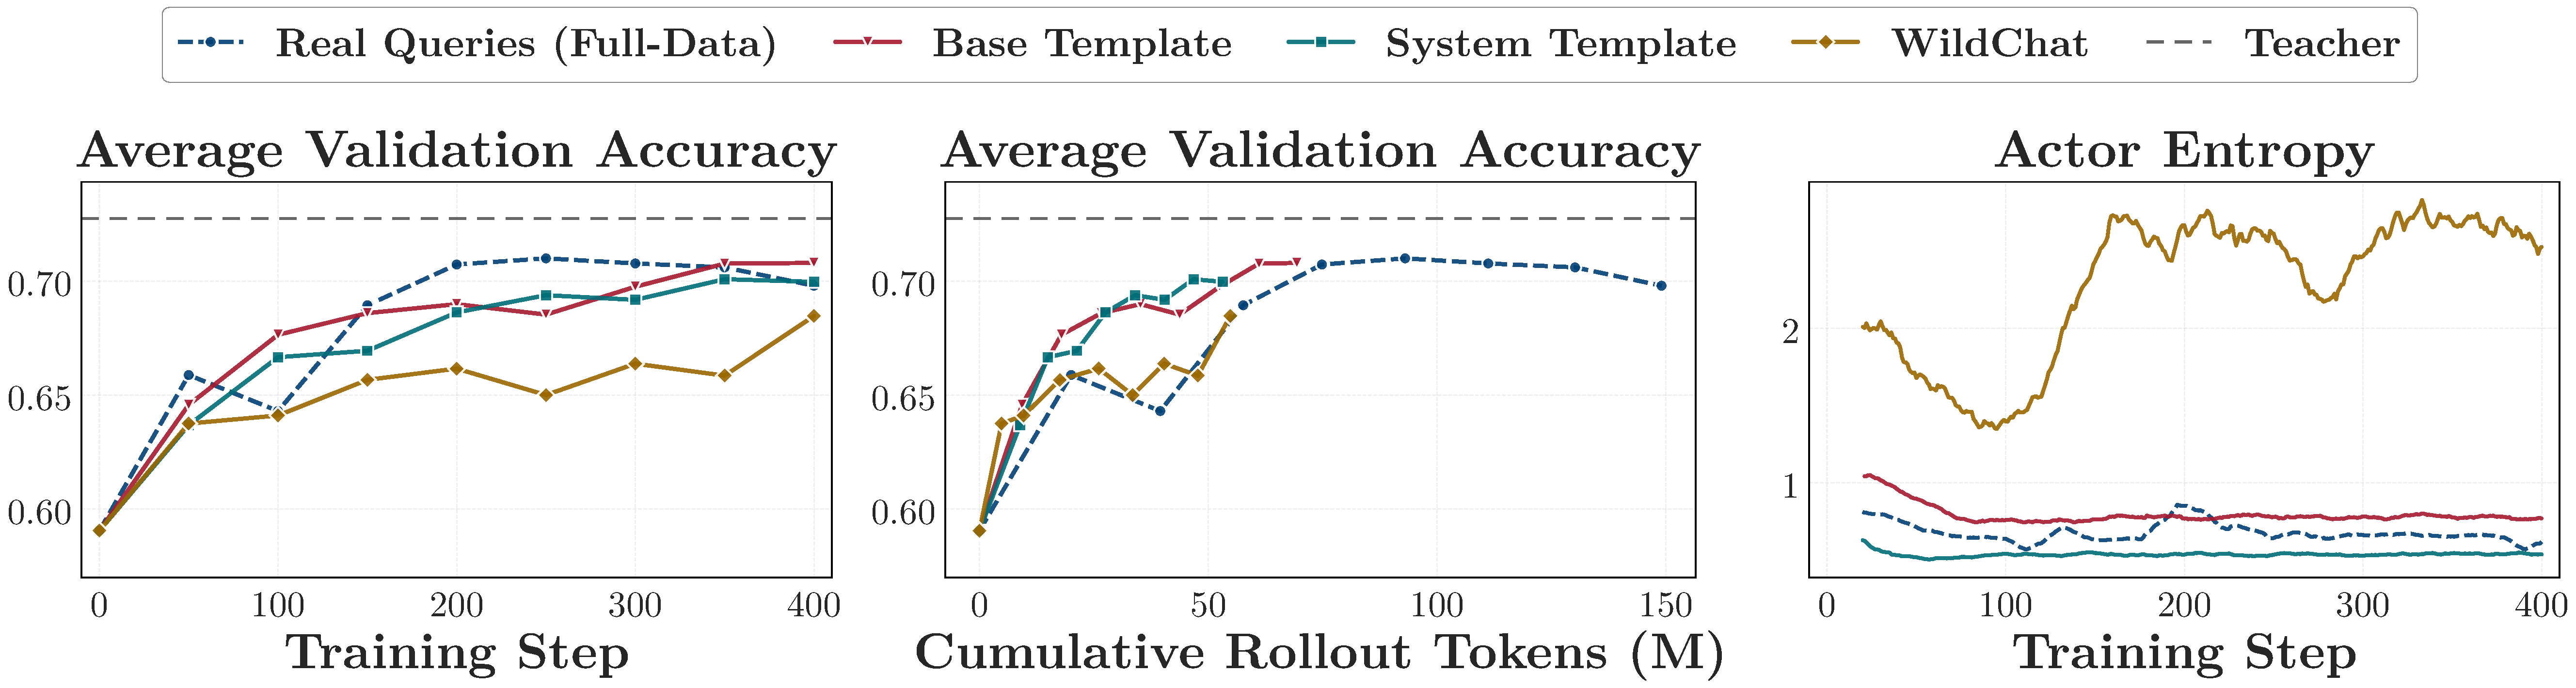
\includegraphics[width=\textwidth]{figures/7_template_wildchat.pdf}
\caption{
在真实训练集、内容较少的模板或通用领域WildChat查询上训练的数学OPD的有效准确率和演员熵。
}
\label{fig:template-wildchat}
\end{figure}

\paragraph{内容稀疏且跨领域的输入仍能引发有用的状态。}
所有三个条件均追踪真实查询基准（real-query baseline），使三个基准的平均值从 \(59.1\) 提升至 \(69.8\)，且三者均在 rollout token 总量的三分之一到二分之一处即达到该水平（图~\ref{fig:template-wildchat}）。代码生成任务亦呈现相同趋势（附录~\ref{app:template-code}）。  
然而，该要求并非空洞：一种能立即闭合该块的支架（scaffold），即 \texttt{<think>\\n}\allowbreak\texttt{</think>\\n}，会坍缩为简短的元层级回复，而此类回复无法用于训练。  
这些结果并不意味着任务内容通常可有可无；相反，它们表明内容并非 OPD 中有用信号的唯一来源。输入本身亦充当状态生成器，即使内容稀疏或来自非目标领域（off-domain）的输入，有时亦可引导学生进入支持有效教师监督（teacher supervision）的状态。在本实验中，显式领域内容（explicit domain content）的改变仅使最终性能波动约一个百分点。这为理解 OPD 的数据效率提供了互补视角：数据质量不仅取决于所收集问题本身，还取决于这些问题所诱导出的状态区域（state regions），以及在这些区域内可获得的教师目标（teacher targets）。

\subsection{与one-shot RLVR的关系}
\label{sec:opd-vs-rlvr}

one-shot OPD 与 one-shot RLVR~\citep{wang2025oneshot} 具有相同的表面现象：单次查询即可支持在 OPD 中经过数百次更新的持续改进，以及在 RLVR 中经过上千次更新的持续改进。其学习来源不同：OPD 在每个访问的状态下接收教师目标，而 RLVR 则为每条轨迹接收可验证的结果。我们通过相同的中等复杂度查询来比较二者，以隔离这一差异（图~\ref{fig:opd-vs-rlvr}）。

\begin{figure}[t]
\centering
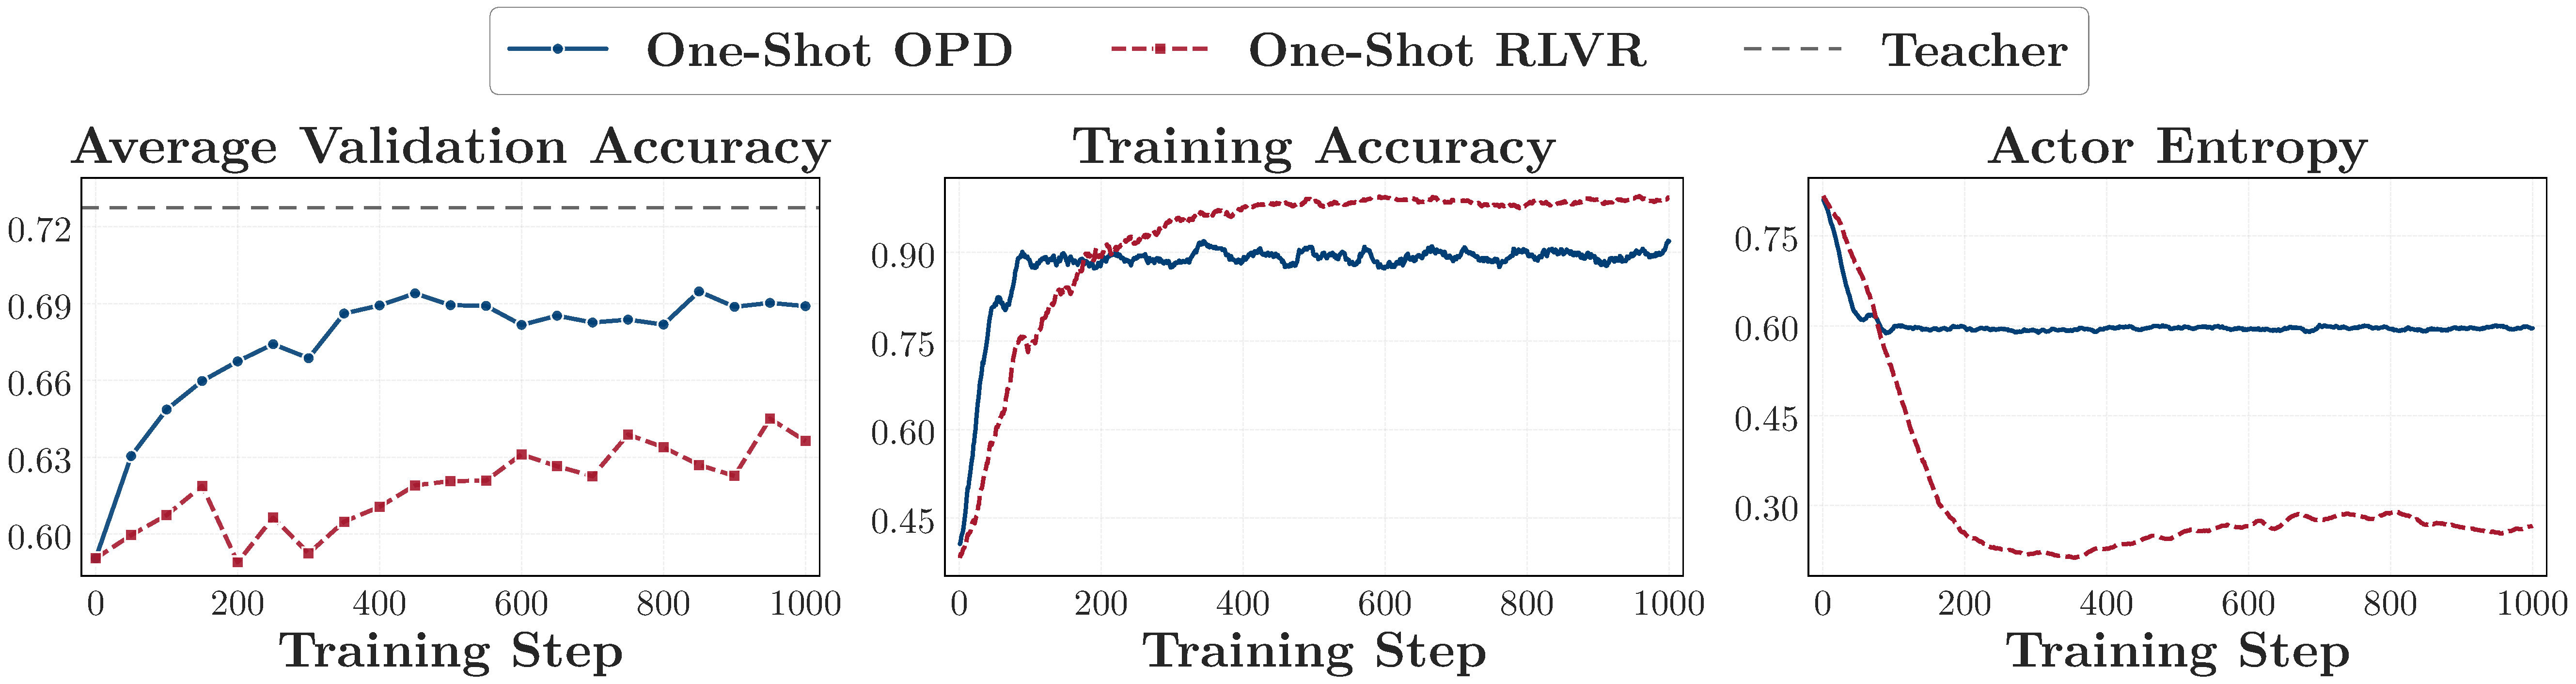
\includegraphics[width=\textwidth]{figures/7_opd_vs_rlvr.pdf}
\caption{
有效准确率和训练动态在相同查询下的 one-shot OPD 与 one-shot RLVR。两者每步均处理批量 \(64\)  查询。RLVR 每个查询抽取 \(8\)  轮次，并根据 GRPO 下的结果对每轮进行评分。OPD 抽取 \(1\)  并对每个采样 token 与教师进行对比评分。训练准确率是解决训练查询的轮次所占比例。
}
\label{fig:opd-vs-rlvr}
\end{figure}

\paragraph{有用的输入因目标而异。}
RLVR 从轨迹结果中进行更新。因此，其训练输入必须定义一个任务，使得采样的结果可以被验证。这些结果还必须具备足够的变化性，以产生有用的优势。而 OPD 则从每个访问状态下的教师-学生差距中进行更新。只要某个提示导致轨迹暴露出此类差距，它就能接收到有用的信号。因此，OPD 输入的价值并不直接依赖于可验证性或难度。我们的结果进一步表明，即使在我们研究的情景中，较弱的领域对齐也能发挥作用。诱导状态区域的覆盖仍然重要（第~\ref{sec:data} 节），但获得这种覆盖所需的限制远低于获得具有可验证结果的任务。

\paragraph{OPD 从同一查询中提取了更多信号。}
两个算法在每一步都从训练查询中获取新的轨迹。在 \(1000\) 步内，OPD 缩小了与教师模型之间差距的 \(72\%\)。其验证准确率的提升是 RLVR 的两倍以上。当两种方法按轨迹 token 数量而非训练步数进行匹配时，这一优势依然存在（图~\ref{fig:opd-vs-rlvr}）。

随着模型学会解决训练查询，RLVR 信号会逐渐减弱。其组别很快变得几乎一致，这使得在 GRPO 下无法获得优势。OPD 不依赖于轨迹结果的变化。即使在查询被解决后，它仍能从局部的教师-学生差距中继续学习，尽管这些差距逐渐缩小。因此，one-shot RLVR 的局限性在于其查询所能提供的结果变化；而 one-shot OPD 的局限性则在于其吸收稠密教师监督的速度，如第~\ref{sec:data} 和~\ref{sec:algorithm} 节所示。此外，两种目标也意味着不同的上限：RLVR 不受教师分布的限制，而 OPD 则被训练以匹配某一特定分布。
